

% Autor: Lukas Deeken
% Letzte Bearbeitung: 22.01.2023

\chapter{Einleitung}

\section{Formula Student}
Die Formula Student ist ein weltweiter Ingenieurswettbewerb bei dem es darum geht das eine Gruppe von Studenten einen Formel Rennwagen nach dem Regelwerk der Formula Student entwirft und baut. Mit diesen Rennwagen wird dann auf den diversen Events in Europa und der ganzen Welt gegen die anderen Teams angetreten. Hierbei gibt es die Verbrenner Kategorie welche in den nächsten Jahren voraussichtlich auslaufen wird und die Elektro Kategorie. Features des Autonomen Fahren werden dabei zusätzlich gewertet wenn vorhanden. Es gibt die statischen Disziplinen, hierbei geht es darum das Design des Autos gegenüber einer Jury zu verteidigen als auch eine detaillierte Kostenaufstellung sowie einen Geschäftsmodell für das Fahrzeug zu liefern. Dann gibt es die dynamischen Disziplinen, hier fahren die Studenten die Fahrzeuge selbst um verschiedene Kurse. Ziel ist immer den Kurs in der kürzesten Zeit zu absolvieren. Die längste Fahretappe ist dabei ein \ensuremath{22 km} Sprint um einen Rundkurs.

\section{Baltic Racing}
Bei dem Formula Student Team in dessen Rahmen diese Arbeit entstanden ist handelt es sich um eines der ältesten Deutschlands. Seit 1999 wurden in diesem Team Fahrzeug mit Verbrennungsmotoren gebaut. Im Jahr 2020 hat die \acfirst{FSG} angekündigt das die Verbrenner Kategorie zum Jahr 2022 bei diesem Event auslaufen wird. In diesem Zuge hat man sich bei Baltic Racing in der 2021er Saison dazu entschieden mit der Entwicklung eines Elektrofahrzeuges zu beginnen. Zu diesem Zeitpunkt ist der Autor dieser Arbeit zum Leiter dieser neuen E-Antriebs Abteilung geworden mit der Aufgabe den ersten E-Antrieb zu konzeptionieren und umzusetzen.

\section{Das Fahrzeug}
An dieser Stelle wird der folgenden Arbeit vorgegriffen und es wird das Ergebnis vorgestellt. Ziel ist das der Leser sich in der folgenden Arbeit besser orientieren kann und so ein Gesamtbild von dem Projekt erlangt.\\
\\
Die Abbildungen \ref{fig:renderingty22front} und \ref{fig:renderingty22rear} zeigen die Gesamtbaugruppe des Fahrzeuges.\\
\\
	\begin{minipage}[b]{.5\linewidth} % [b] => Ausrichtung an \caption
			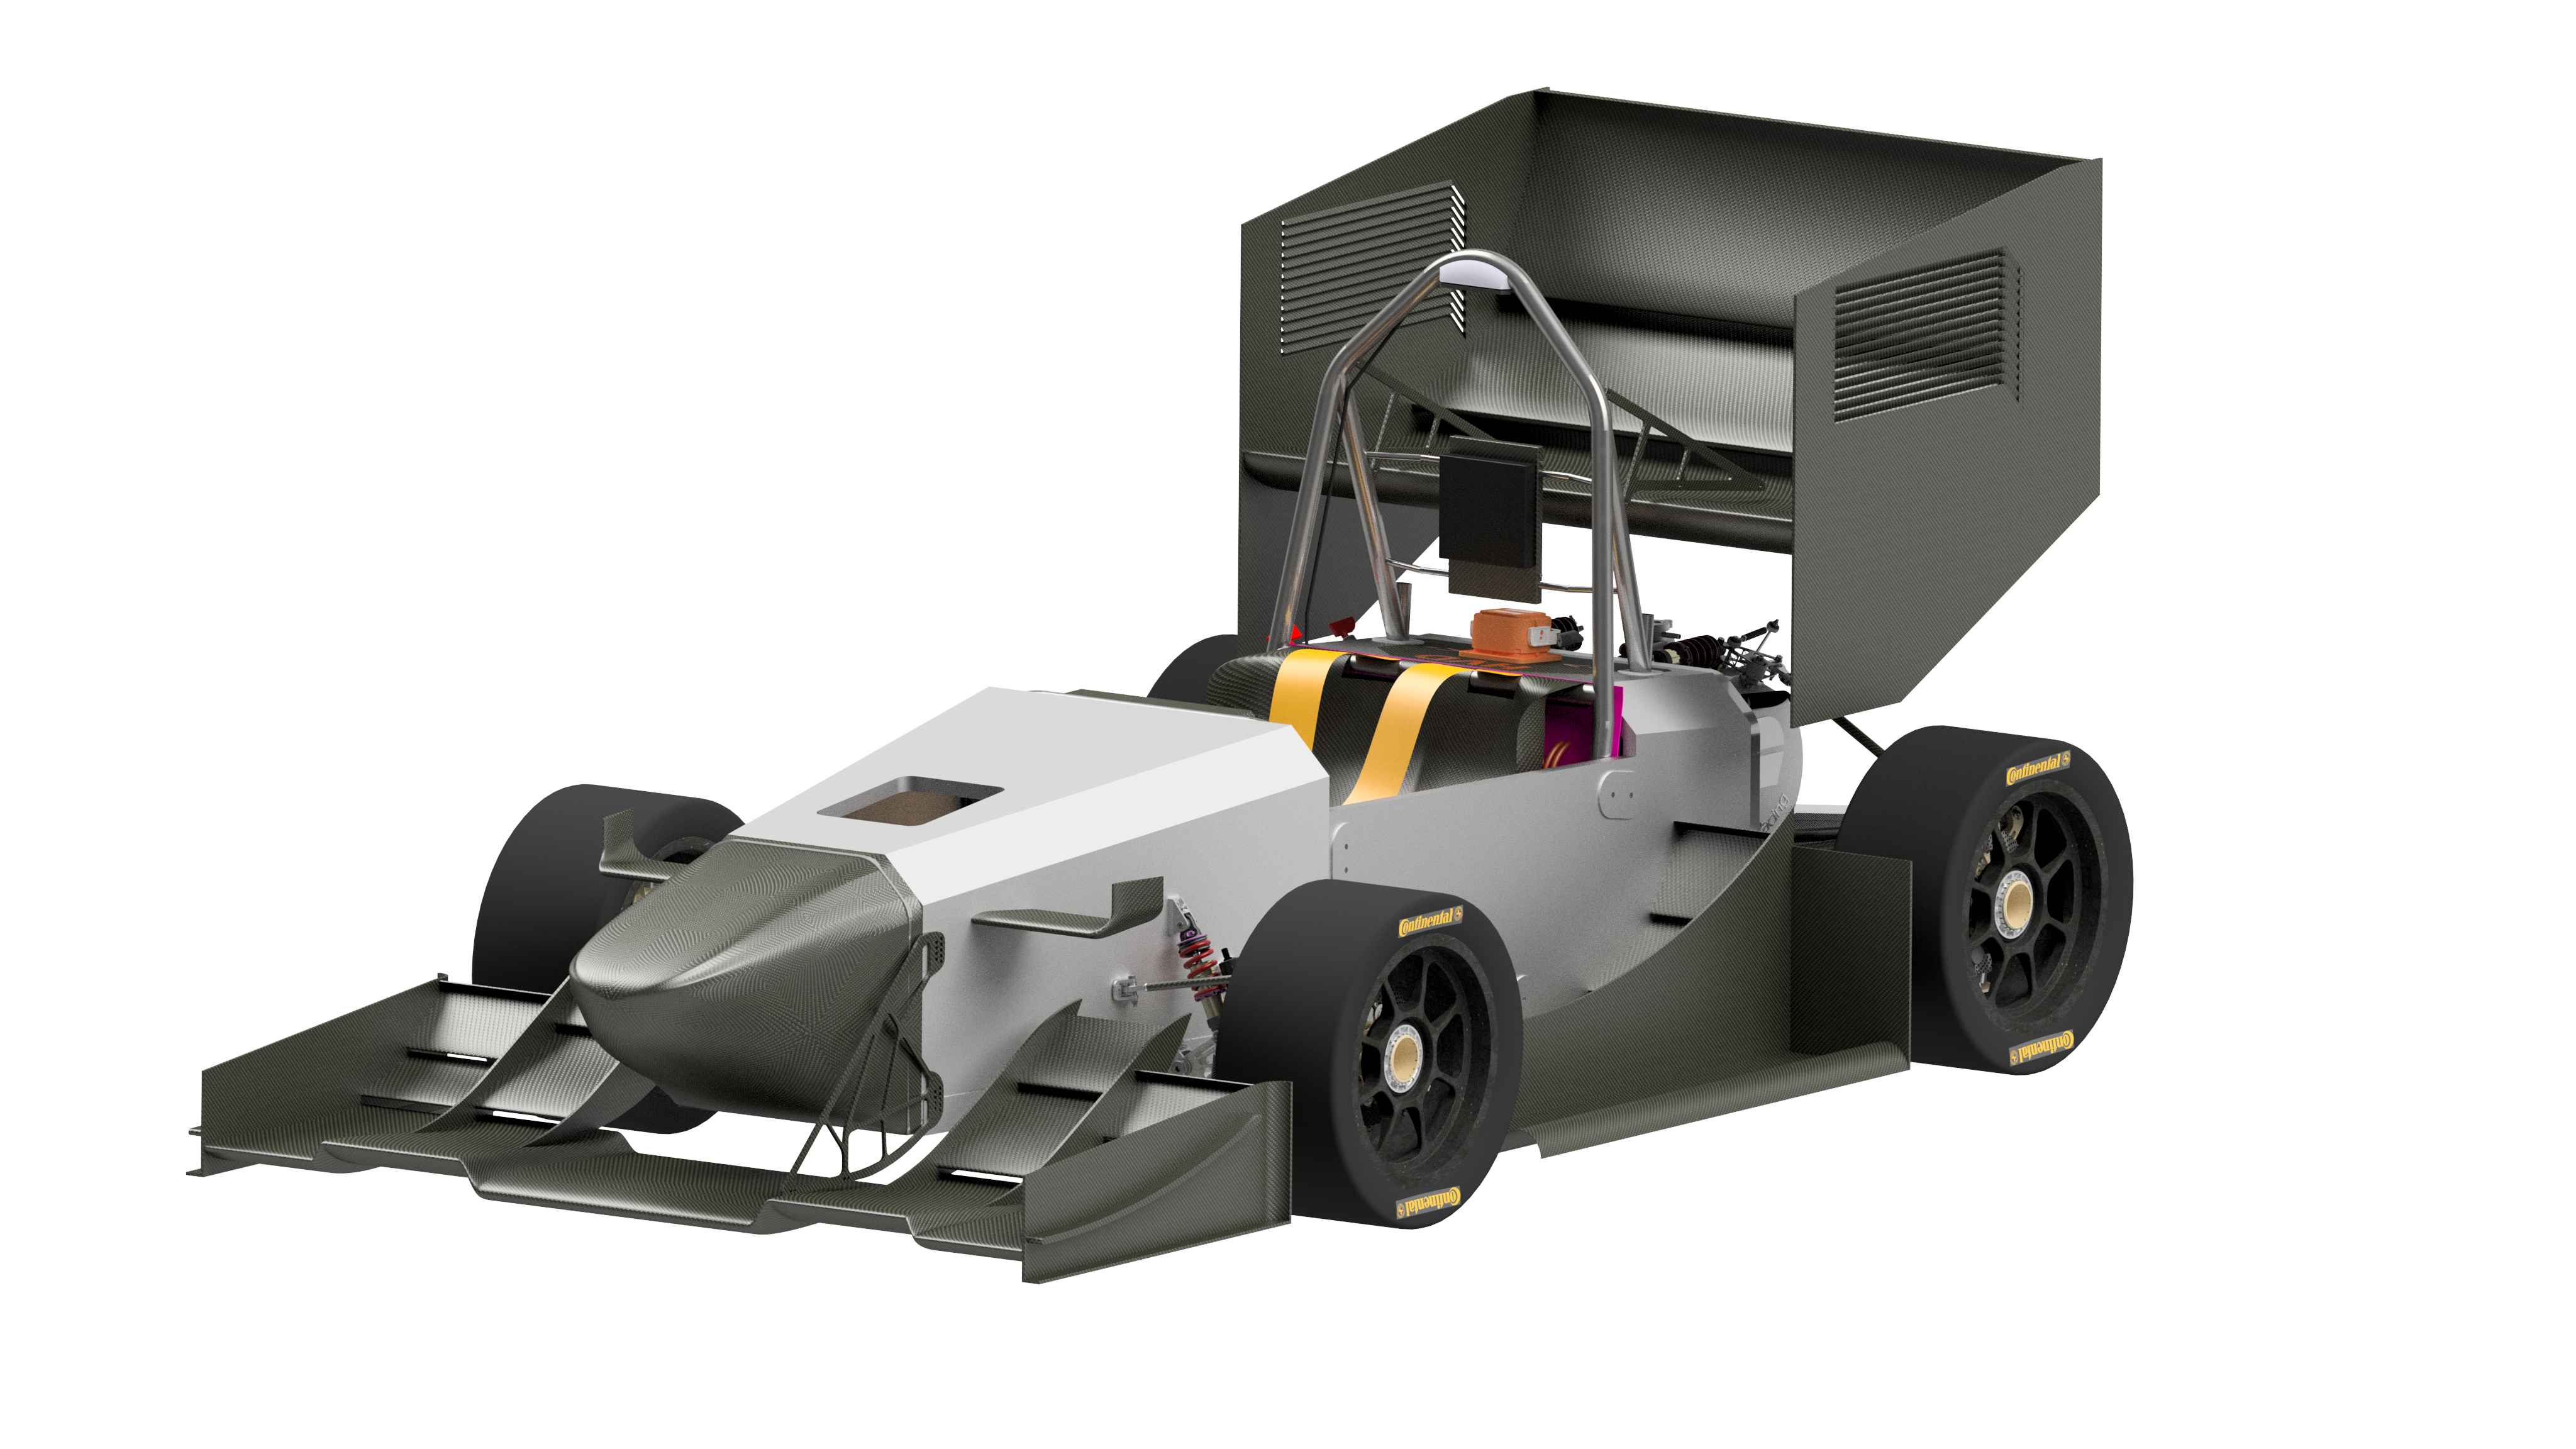
\includegraphics[width=1\linewidth]{bilder/Rendering_TY22_Front}
			\captionof{figure}{TY22 Iso Vorne}
			\label{fig:renderingty22front}
	\end{minipage}
	\begin{minipage}[b]{.5\linewidth} % [b] => Ausrichtung an \caption
			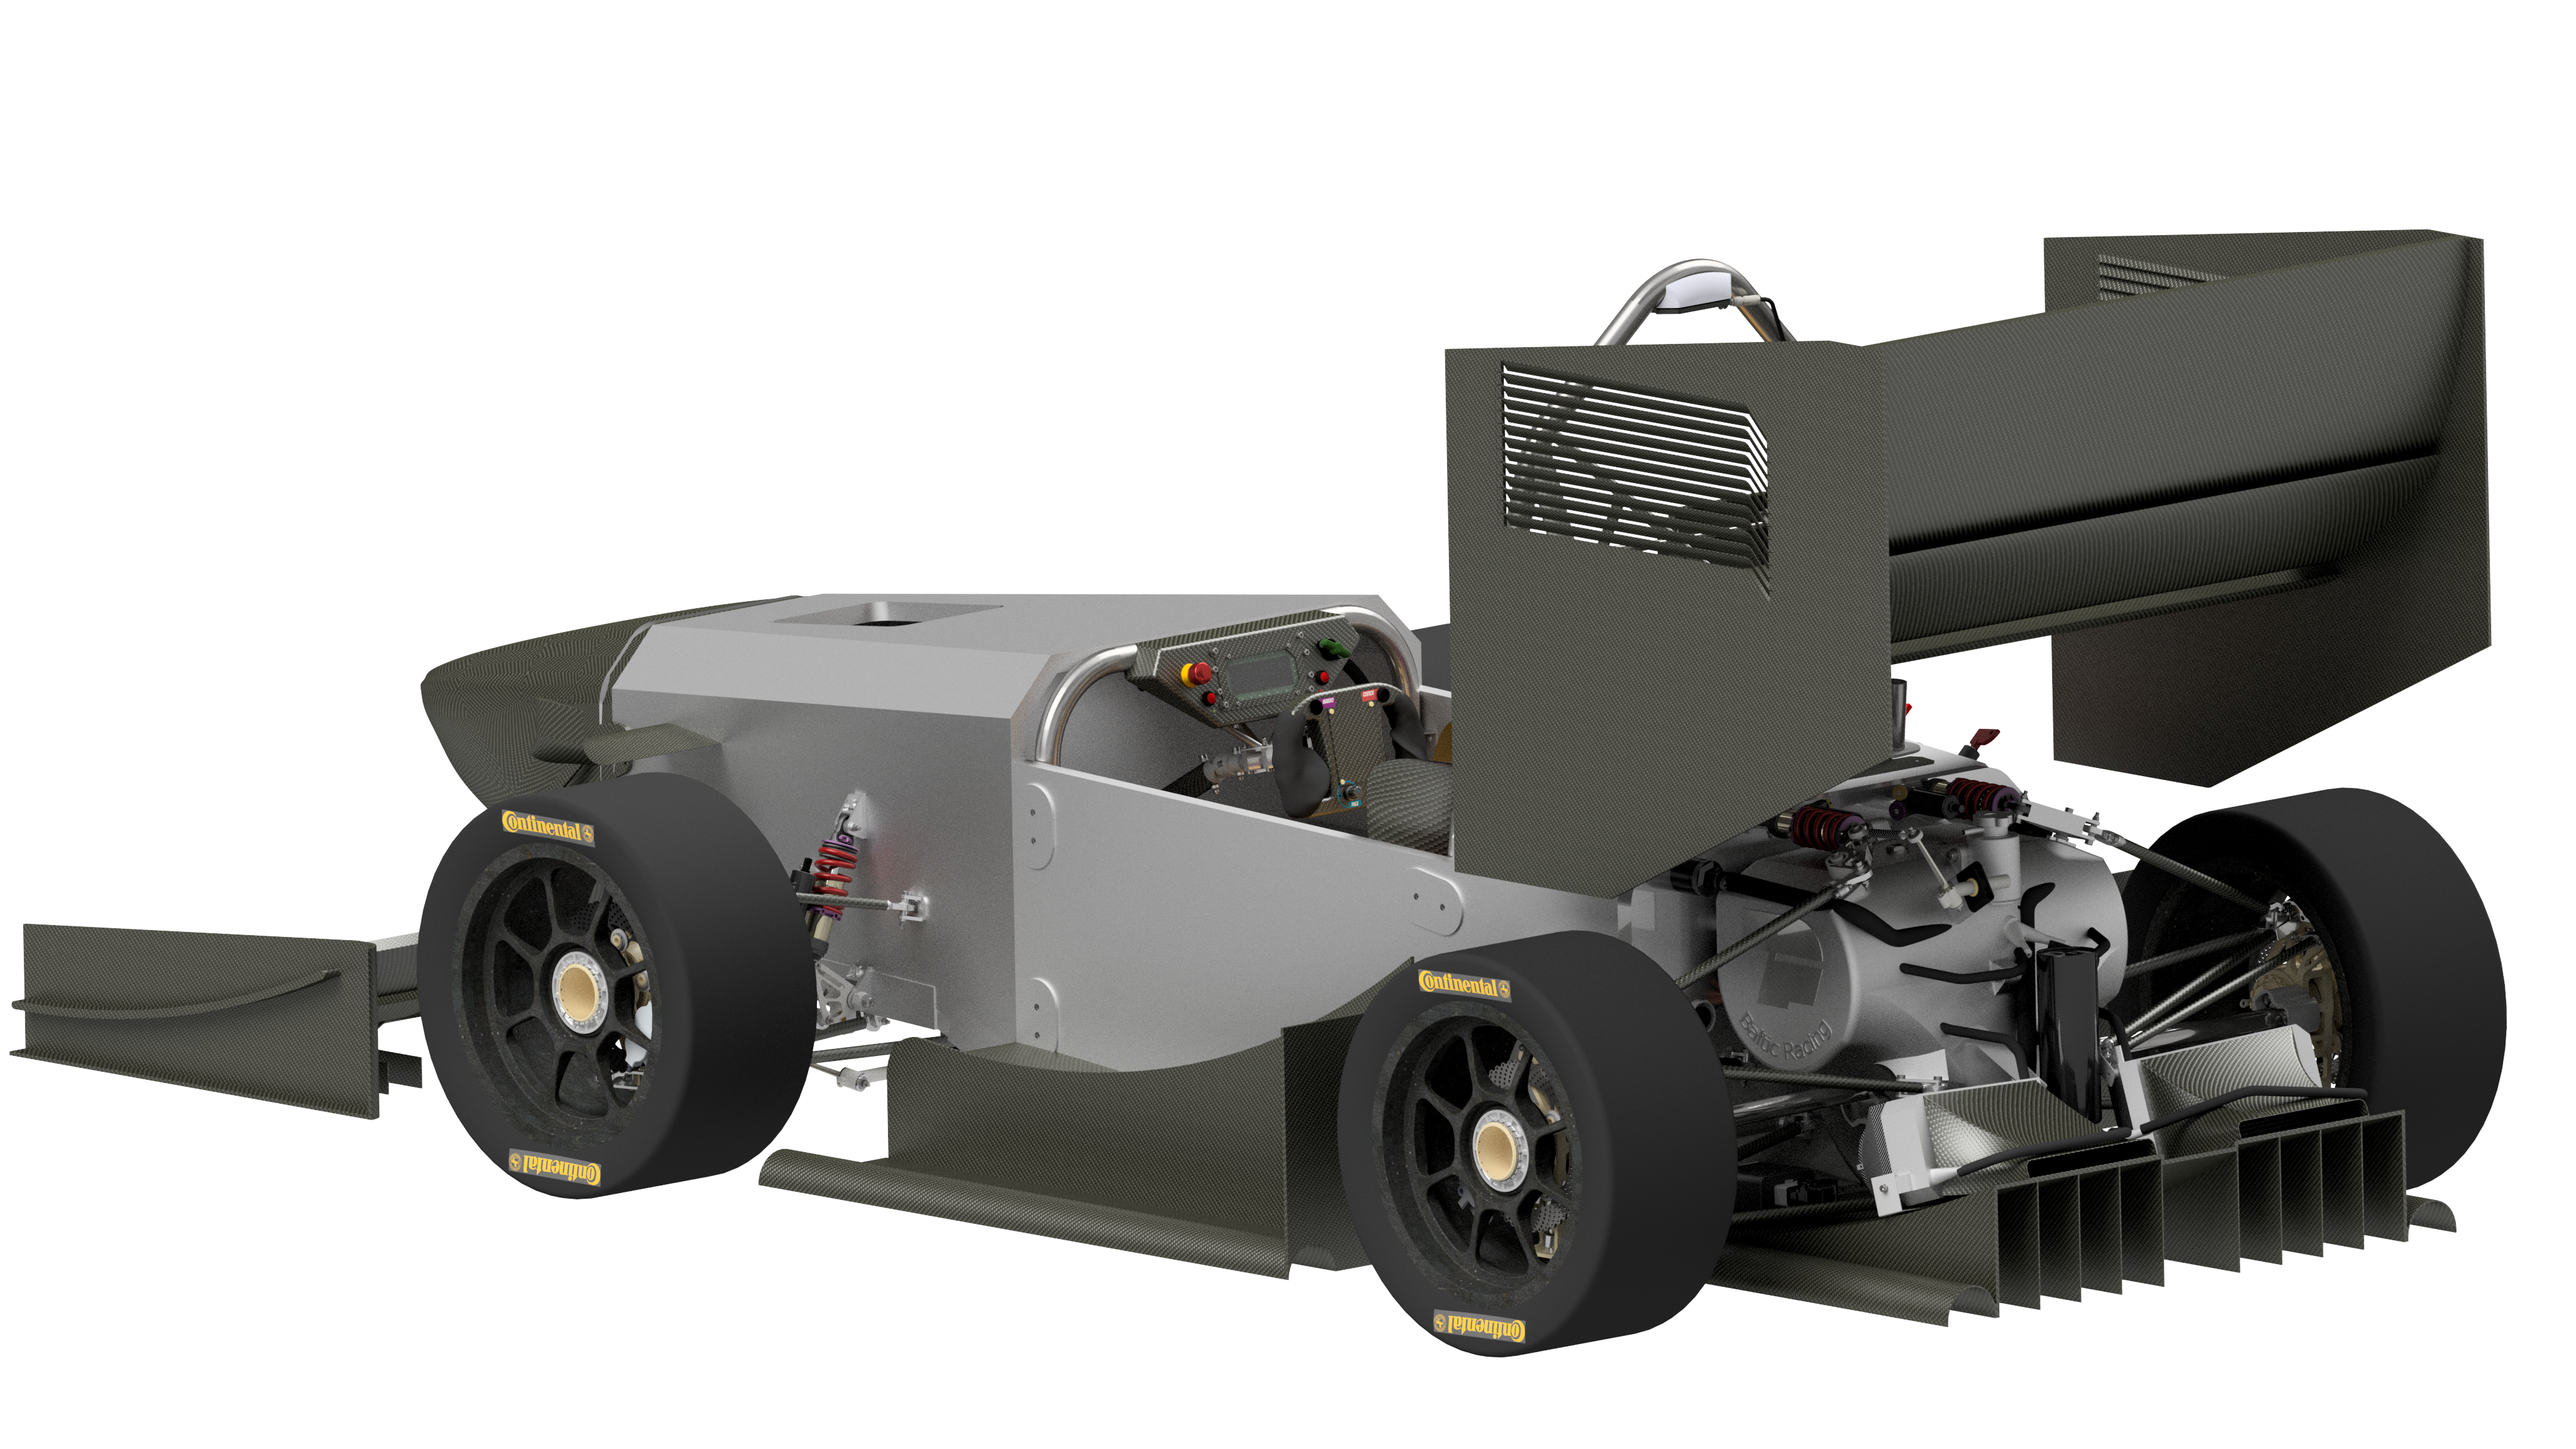
\includegraphics[width=1\linewidth]{bilder/Rendering_TY22_Rear}
			\captionof{figure}{TY22 Iso Hinten}
			\label{fig:renderingty22rear}
	\end{minipage}

Die Abbildung \ref{fig:epowertrainassemblyv4} zeigt die Gesamtbaugruppe des E-Antriebes isoliert von den restlichen Komponenten.\\
\\
Bei dem Antriebslayout handelt es sich um einen Zweirad Antrieb auf der Hinterachse mit jeweils einem Elektromotor und einer Getriebestufe pro Rad. Bei dem Getriebe handelt es sich um eine Einstufige Stirnraduntersetzung, mit einer Untersetzung von 4,32 in einem Aluminiumgussgehäuse. Hierbei umfasst das Gehäuse sowohl die Getriebestufe als auch die Elektromotoren. Die Elektromotoren sind Kaufteile der Firma Emrax, es handelt sich um den Emrax 208. Nebst den Antriebskomponenten ist auch das hintere Fahrwerk an diesem Gehäuse angebracht und stellt so einen tragenden Teil der Karosserie dar. Der Akku ist möglichst flach und breit gebaut und befindet sich an der tiefsten Stelle im Chassis schräg hinter/unter dem Fahrer. Verwendet werden Rundzellen im Format 18650, welche liegend in Akkugehäuse untergebracht sind. Bei dem Gehäuse handelt es sich um eine Aluminium Schweißkonstruktion. Der Akku hat eine Gesamtkapazität von \ensuremath{7,4 kWh} bei einem Gesamtgewicht von ca. \ensuremath{45 Kg} Neben den Zellen befindet es hier auch die restliche Akku-relevante Elektronik. Über dem Akkumulator befinden sich die Umrichter. Hierbei handelt es sich um zugekaufte Teile der Firma Drivetrain Innovations. Über den Umrichtern befindet sich die \ac{HV}-Verteilerbox. Hier ist sämtliche übrige \ac{HV} Elektronik untergebracht. Die Radiatoren befinden sich am hintersten Teil des Fahrzeuges auf dem Diffusor und leiten die warme Abluft über den Diffusor. Für die Lüfter wurden Drohnen/-Motoren und -Propeller eingesetzt.

\begin{figure}
	\centering
	\includegraphics[width=1\linewidth]{bilder/E_powertrain_Assembly_V4.2}
	\caption{E-Antrieb Gesamtbaugruppe}
	\label{fig:epowertrainassemblyv4}
\end{figure}

\FloatBarrier